\documentclass[a4paper,11pt,titlepage]{jsarticle}
\usepackage[final]{graphicx}
\usepackage[dvipdfmx]{color}
\usepackage{listings, xcolor}
\usepackage{amsmath}
\usepackage{here}
\usepackage{tikz}
\usepackage{subcaption}

\lstset{
    basicstyle = {\ttfamily},
    frame = {tbrl},
    breaklines = true,
    numbers = left,
    showspaces = false,
    showstringspaces = false,
    showtabs = false,
    keywordstyle = \color{blue},
    commentstyle = {\color[HTML]{1AB91A}},
    identifierstyle = \color{black},
    stringstyle = \color{brown},
    captionpos = t
}

\title{画像処理レポート4}
\author{235738B 越後 玲輝}

\begin{document}

\maketitle
\newpage

\section{平均化フィルタの調査}
教科書P.107図5.5の加重平均化フィルタ(3x3)および(5x5)と、


P.106図5.3の平均化フィルタ(3x3)および(5x5)を、任意の
画像に適用し、それぞれのフィルタの効果を”比較検討”しなさい。


違いがわかるような適切な比較検討方法ないし実験を自由に
考案して実施。

\subsection{ソースコード}
\begin{figure}[htbp]
\centering
\lstinputlisting[caption={平均化フィルタ}, label={lst:unsharp}]{rep4-4.py}
\end{figure}

\begin{figure}[htbp]
\centering
\lstinputlisting[caption={ガウシアンフィルタ}, label={lst:unsharp}]{/Users/reiki/workSpace/imageStu/report4/rep4-4-gaus.py}
\end{figure}


\clearpage

\subsection{出力画像}

\begin{figure}[htbp]
  \centering

  \begin{subfigure}{0.4\textwidth}
    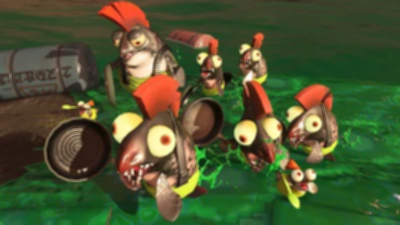
\includegraphics[width=\linewidth]{syake_filter3x3.png}
    \caption{平均化フィルタ 3×3}
  \end{subfigure}
  \hfill
  \begin{subfigure}{0.4\textwidth}
    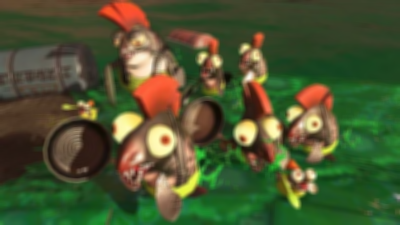
\includegraphics[width=\linewidth]{syake_filter5x5.png}
    \caption{平均化フィルタ 5×5}
  \end{subfigure}

  \vspace{2mm}

  \begin{subfigure}{0.4\textwidth}
    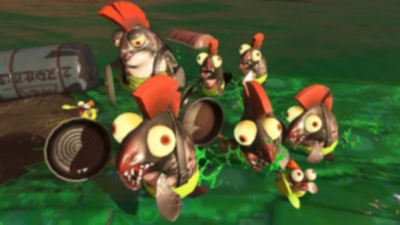
\includegraphics[width=\linewidth]{syake_filter_Gauss_3x3.png}
    \caption{ガウシアンフィルタ 3×3}
  \end{subfigure}
  \hfill
  \begin{subfigure}{0.4\textwidth}
    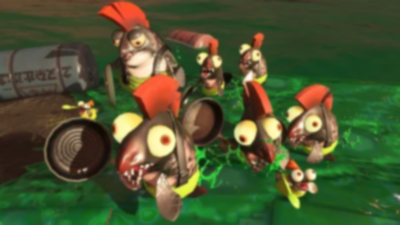
\includegraphics[width=\linewidth]{syake_filter_Gauss_5x5.png}
    \caption{ガウシアンフィルタ 5×5}
  \end{subfigure}

  \caption{4種類のフィルタ比較}
\end{figure}

\subsection{比較、目視での画像確認}

図1に示したように、同一の入力画像に対して4種類の平滑化フィルタを適用し、その効果を比較した。

(a) 平均化フィルタ 3×3 は、ノイズ除去効果は控えめだが、輪郭が比較的保たれており、元画像の情報を大きく損なわない処理となった。

(b) 平均化フィルタ 5×5 では、より広範囲にわたって平均化されるため、全体的にぼやけた印象となった。特にキャラクターの顔や背景の輪郭が著しく失われており、ノイズ除去には有効だが、情報損失も大きい。

(c) ガウシアンフィルタ 3×3 は、平均化と比べて中央に重みを持つため、エッジ部分の情報がより保持され、滑らかさとディテールの両立が見られた。実用上のバランスに優れる。

(d) ガウシアンフィルタ 5×5 では、より強く滑らかに処理され、背景やノイズは効果的に除去されているものの、キャラクターの輪郭もややぼやけている。視認性は高いが、情報保持には注意が必要である。

以上の比較から、ガウシアンフィルタは平均化フィルタよりも滑らかさと情報保持のバランスに優れ、特に3×3サイズは最も自然な視覚効果を与えることを体感した。


\section{鮮鋭化フィルタの調査}
教科書P.123の可変鮮鋭化フィルタを任意の画像に適用し、その効果を
調べなさい。

効果の違いがわかるような適切な比較検討方法
ないし実験を自由に考案して実施。

\subsection{ソースコード}
\lstinputlisting{rep4-5.py}

\subsection{出力画像}

\begin{figure}[htbp]
  \centering

  \begin{subfigure}{0.4\textwidth}
    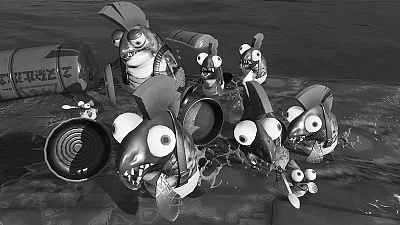
\includegraphics[width=\linewidth]{syake_unsharp_masked_3x3_k=1.png}
    \caption{鮮鋭化フィルタ k=1}
  \end{subfigure}
  \hfill
  \begin{subfigure}{0.4\textwidth}
    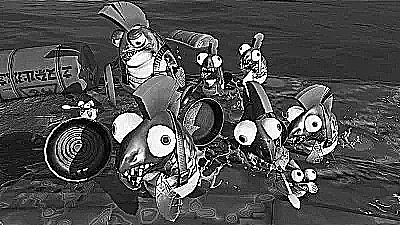
\includegraphics[width=\linewidth]{syake_unsharp_masked_3x3_k=10.png}
    \caption{鮮鋭化フィルタ k=10}
  \end{subfigure}

  \vspace{2mm}

  \begin{subfigure}{0.4\textwidth}
    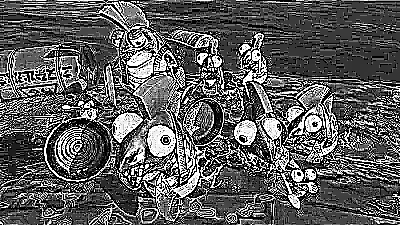
\includegraphics[width=\linewidth]{syake_unsharp_masked_3x3_k=50.png}
    \caption{鮮鋭化フィルタ k=50}
  \end{subfigure}
  \hfill
  \begin{subfigure}{0.4\textwidth}
    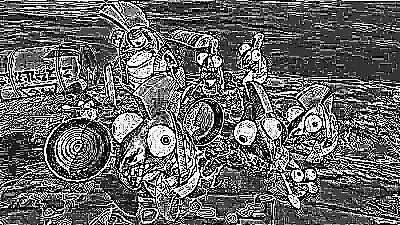
\includegraphics[width=\linewidth]{syake_unsharp_masked_3x3_k=100.png}
    \caption{鮮鋭化フィルタ k=100}
  \end{subfigure}

  \caption{kの値を変化、比較}
\end{figure}

\subsection{比較、目視での画像確認}

図2に示したように、係数 $k$ の値を変化させることで、鮮鋭化の強さが大きく異なることがわかる。

(a) の $k=1$ では、エッジがほどよく強調され、画像全体の視認性が向上しているが、不自然さはない。バランスの取れた出力である。

(b) の $k=10$ では、鮮鋭化が強くなり、細部がさらに明瞭になるが、背景の一部にノイズが目立ち始めた。鮮鋭化の効果が強く出る一方で、画像としての自然さはやや損なわれる。

(c) の $k=50$ および (d) の $k=100$ では、エッジが過剰に強調され、画像全体が輪郭線だらけのような印象となった。特に $k=100$ では、画像としての再利用が困難なほど情報が劣化している。

この結果から、$k$ の値は画像の目的に応じて適切に設定する必要がある。一般的な使用では、$k=1$ 〜 $5$ 程度が妥当であり、それ以上では鮮鋭化による副作用(ノイズ増強、視認性低下)が顕著となることが確認された。

\section{輪郭抽出}
任意の画像から輪郭を抽出しなさい。できるだけ綺麗な輪郭を抽出
すること。

そのためにどのような工夫や処理を行ったか結果・コード
とともに記述すること。

\subsection{ソースコード}
\lstinputlisting[caption={輪郭抽出}, label={lst:unsharp}]{rep4-6.py}

\subsection{出力画像}

\begin{figure}[htbp]
  \centering
  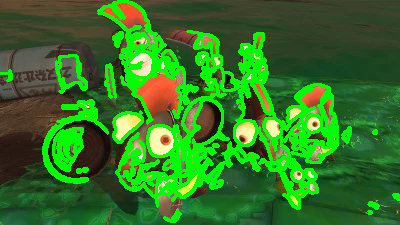
\includegraphics[width=0.4\linewidth]{syake_contours.png}
  \caption{輪郭抽出結果}
  \label{fig:contour}
\end{figure}


\subsection{輪郭抽出における工夫}

輪郭をできるだけ綺麗に抽出するために、以下のような前処理およびパラメータ調整を行った。

\begin{itemize}
  \item \textbf{ノイズ除去のための前処理}として、入力画像に対してガウシアンフィルタを適用した。
  
  これにより、Canny法における誤検出(偽エッジ)を抑制し、安定した輪郭抽出が可能。
  
  \item \textbf{Cannyエッジ検出}を用いて、画素値の急激な変化を抽出した。閾値は \texttt{threshold1=100}, \texttt{threshold2=200} に設定し、細部のエッジは除外しつつも主要な構造が抽出されるように調整。
  
  \item \textbf{外輪郭のみを抽出するために}、 \texttt{cv2.findContours()} のモードとして \texttt{cv2.RETR\_EXTERNAL} を使用した。これにより、内部構造のノイズや細かい輪郭を排除し、視認性の高い主要な輪郭だけを残すことができた。
  
  \item 輪郭描画には \texttt{cv2.drawContours()} を使用し、元画像(カラー)に対して緑色の線で描画した。これにより、元画像の情報を保ちつつ、輪郭の強調部分が一目でわかるように工夫した。
\end{itemize}

これらの工夫により、過剰なノイズを含まず、対象物の輪郭が明確に抽出された画像を得ることができた。特に、前処理としてのガウシアンフィルタと、輪郭の絞り込みとしての \texttt{RETR\_EXTERNAL} の組み合わせが個人的に気に入っている。

\section{周波数フィルタ(ローパスフィルタ)を任意の画像に適用}
\subsection{ソースコード}
\lstinputlisting{rep4-7.py}

\subsection{出力画像}

\begin{figure}[htbp]
  \centering

  \begin{subfigure}{0.4\textwidth}
    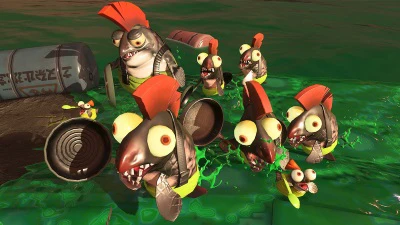
\includegraphics[width=\linewidth]{syake_image.png}
    \caption{ローパスフィルタ前}
  \end{subfigure}
  \hfill
  \begin{subfigure}{0.4\textwidth}
    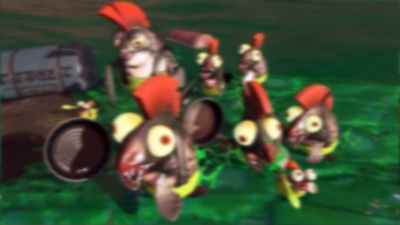
\includegraphics[width=\linewidth]{syake_lowpass_filter.png}
    \caption{ローパスフィルタ後}
  \end{subfigure}

  \caption{ローパスフィルタ実行結果}
\end{figure}

\subsection{ローパスフィルタの効果}

図4に示すように、ローパスフィルタ適用後の画像では全体的にエッジがなだらかになり、シャープな輪郭がぼけた状態となっている。これは高周波成分(ディテール)が除去されたことを示しており、ノイズ除去や滑らかさ向上の効果が出ていることがわかる。

この処理は、プリプロセッシング(前処理)としてノイズ軽減に用いることができる。





\end{document}
